%%%%%%%%%%%%%%%%%%%%%%%%%%%%%%%%%%%%%%%%%%%%%%%%%%%%%%%%%%%%%%%%%%%%%%
% LaTeX Template: Two Column Colour Article
%
% Source: http://www.howtotex.com/
% Feel free to distribute this template, but please keep the
% referal to howtotex.com.
% Date: Feb 2011
% 

%%% Preamble
\documentclass[	DIV=calc,%
paper=a4,%
fontsize=11pt,%
twocolumn]{scrartcl} % KOMA-article class

\usepackage{lipsum}	% Package to create dummy text
\usepackage[english]{babel}	% English language/hyphenation
\usepackage[protrusion=true,expansion=true]{microtype}	% Better typography
\usepackage{amsmath,amsfonts,amsthm} % Math packages
\usepackage[pdftex]{graphicx} % Enable pdflatex
\usepackage{wrapfig} % enable figure wrapping
\usepackage[svgnames]{xcolor} % Enabling colors by their 'svgnames'
\usepackage[hang, small,labelfont=bf,up,textfont=it,up]{caption} % Custom captions under/above floats
\usepackage{epstopdf} % Converts .eps to .pdf
\usepackage{subfig}	% Subfigures
\usepackage{booktabs} % Nicer tables
\usepackage{fix-cm}	% Custom fontsizes
\usepackage{booktabs} % prof. looking tables (www.en.wikibooks.org/wiki/LaTeX/Tables#Professional_tables)
\usepackage{tikz}
\usepackage{amsmath}
\usetikzlibrary{quotes,angles}
\usepackage{mathtools}
\usepackage{tkz-euclide}
\usetikzlibrary{decorations.pathreplacing}
\usepackage{svg}

%%% Custom sectioning (sectsty package)
\usepackage{sectsty} % Custom sectioning (see below)
\allsectionsfont{%		% Change font of al section commands
	\usefont{OT1}{phv}{b}{n}%	% bch-b-n: CharterBT-Bold font
}

\sectionfont{%		% Change font of \section command
	\usefont{OT1}{phv}{b}{n}%	% bch-b-n: CharterBT-Bold font
}


%%% Headers and footers
\usepackage{fancyhdr} % Needed to define custom headers/footers
\pagestyle{fancy} % Enabling the custom headers/footers
\usepackage{lastpage}	

% Header (empty)
\lhead{}
\chead{}
\rhead{\today}
% Footer (you may change this to your own needs)
\lfoot{\footnotesize \texttt{Math Notes for ML} \textbullet ~ Bhargav}
\cfoot{}
\rfoot{\footnotesize page \thepage\ of \pageref{LastPage}}	% "Page 1 of 2"
\renewcommand{\headrulewidth}{0.0pt}
\renewcommand{\footrulewidth}{0.4pt}
\newcommand{\hformbar}[1]{\vspace{5pt}\hrule\vspace{10pt}} % creates a horizontal bar to separate formulae better; space adaptions can be made centrally here


%%% Creating an initial of the very first character of the content
\usepackage{lettrine}
\newcommand{\initial}[1]{%
	\lettrine[lines=3,lhang=0.3,nindent=0em]{
		\color{DarkGoldenrod}
		{\textsf{#1}}}{}}

%%% Title, author and date metadata
\usepackage{titling} % For custom titles

\newcommand{\HorRule}{\color{DarkGoldenrod}%	% Creating a horizontal rule
	\rule{\linewidth}{1pt}%
}

\pretitle{\vspace{-30pt} \begin{flushleft} \HorRule 
		\fontsize{20}{20} \usefont{OT1}{phv}{b}{n} \color{DarkRed} \selectfont 
	}
	\title{Linear Algebra + Stats + Probability Notes} % Title of your article goes here
	\posttitle{\par\end{flushleft}\vskip 0.5em}

\preauthor{\begin{flushleft}\large \lineskip 0.5em \usefont{OT1}{phv}{b}{sl} \color{DarkRed}}
	\author{Bhargav}	% Author name goes here
	\postauthor{\footnotesize \usefont{OT1}{phv}{m}{sl} \color{Black} \hspace{5pt} github.com/brpy \par\end{flushleft}\HorRule}

\date{\today} % No date

%%% wws: create a non-indented formula name
\newcommand{\formdesc}[1]{\noindent\textbf{#1}}

% A 2x2 shape matrix
\newcommand{\tctmat}[4]{\begin{bmatrix}
		$#1$ & $#2$\\
		$#3$ & $#4$
\end{bmatrix}}

% A 2x1 shape matrix
\newcommand{\tcomat}[2]{\begin{bmatrix}
		$#1$\\
		$#2$
\end{bmatrix}}

% A 3x3 shape matrix
\newcommand{\thcthmat}[9]{\begin{bmatrix}
		$#1$ & $#2$ & $#3$\\
		$#4$ & $#5$ & $#6$\\
		$#7$ & $#8$ & $#9$
\end{bmatrix}}

% A 3x1 shape matrix
\newcommand{\thcomat}[3]{\begin{bmatrix}
		$#1$\\
		$#2$\\
		$#3$
\end{bmatrix}}

%%% Begin document -----------------------------------------------------------------
\begin{document}
	\maketitle
	\thispagestyle{fancy} 	% Enabling the custom headers/footers for the first page 
	% The first character should be within \initial{}
	\subsection{Linear Algebra:}
	
	\textbf{The following notes is primarily made for my revision. I might have skipped some topics that seemed obvious to me. I do not guarantee factual correctness of the notes. If you feel there are any errors, open a github issue/pr. Notes material is collected from various sources. Image credits are given in tex document and in src.csv}
	
	\hspace{10pt}

\hformbar
\formdesc{Vectors:}

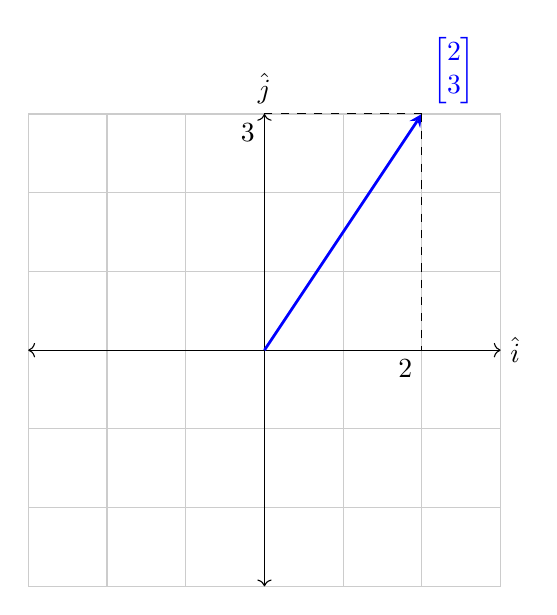
\begin{tikzpicture}
	\draw[thin,gray!40] (-3,-3) grid (3,3);
	\draw[<->] (-3,0)--(3,0) node[right]{$\hat{i}$};
	\draw[<->] (0,-3)--(0,3) node[above]{$\hat{j}$};
	\draw[line width=1pt,blue,-stealth](0,0)--(2,3) node[anchor=south west]{$\boldsymbol{\tcomat{2}{3}}$};
	\draw [dashed] (2,3)--(2,0) node[anchor=north east]{${2}$};
	\draw [dashed] (2,3)--(0,3) node[anchor=north east]{${3}$};
\end{tikzpicture}
\begin{itemize}
	\item This vector is represented as $2\hat{i} + 3\hat{j}$ where $\hat{i}$ and $\hat{j}$ are unit vectors perpendicular to each other also known as basis vectors (in 2d).
	\item It is also represented as a column matrix $\tcomat{2}{3}$
	\item A vector is represented by its length and direction wrto. basis vectors $\hat{i}$, $\hat{j}$.
	\item A vector can be freely moved without changing its length and the direction it is pointing to.
	\item So any vector in space can be represented using a linear combination of $\hat{i}$, $\hat{j}$ by moving the starting point to origin.
\end{itemize}

\hformbar
\formdesc{Adding 2 Vectors:}

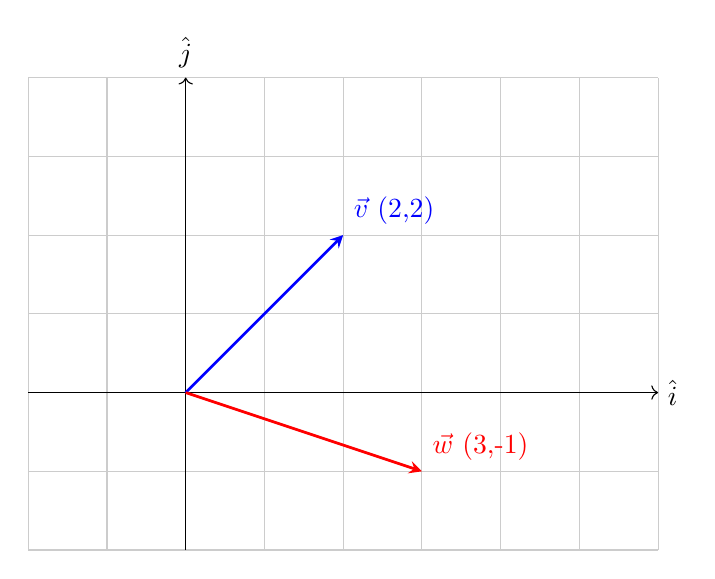
\begin{tikzpicture}
	\draw[thin,gray!40] (-2,-2) grid (6,4);
	\draw[.->] (-2,0)--(6,0) node[right]{$\hat{i}$};
	\draw[.->] (0,-2)--(0,4) node[above]{$\hat{j}$};
	\draw[line width=1pt,blue,-stealth](0,0)--(2,2) node[anchor=south west]{$\vec{v}$	(2,2)};
	\draw[line width=1pt,red,-stealth](0,0)--(3,-1) node[anchor=south west]{$\vec{w}$	(3,-1)};
\end{tikzpicture}

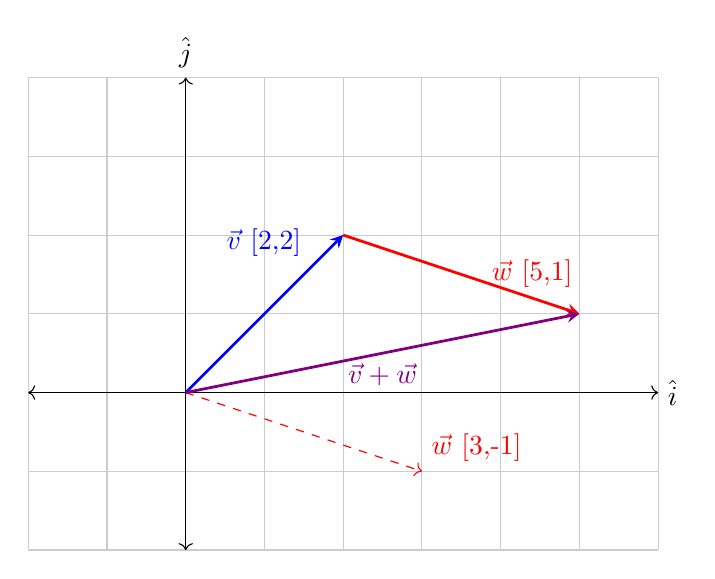
\begin{tikzpicture}
	\draw[thin,gray!40] (-2,-2) grid (6,4);
	\draw[<->] (-2,0)--(6,0) node[right]{$\hat{i}$};
	\draw[<->] (0,-2)--(0,4) node[above]{$\hat{j}$};
	\draw[line width=1pt,blue,-stealth](0,0)--(2,2) node[anchor=south east, pos=0.8]{$\vec{v}$	[2,2]};
	\draw[red, dashed, ->](0,0)--(3,-1) node[anchor=south west]{$\vec{w}$	[3,-1]};
	\draw[line width=1pt,red,-stealth](2,2)--(5,1) node[anchor=south, pos=0.8]{$\vec{w}$	 [5,1]};
	\draw[line width=1pt,violet,-stealth](0,0)--(5,1) node[anchor=north, pos=0.5]{$\vec{v} + \vec{w}$};
\end{tikzpicture}
This is also known as Triangular law of vector addition.




\begin{itemize}
	\item Can also be interpreted as,
	
	
	$\boldsymbol{\tcomat{5}{1}}$ = $\boldsymbol{\tcomat{2}{2}}$ + $\boldsymbol{\tcomat{3}{-1}}$
	\item The vector $\vec{w}$ is moved along $\vec{v}$ such that the starting point of $\vec{w}$ meets the end point of $\vec{v}$
	\item Both $\vec{v}$ and $\vec{w}$ direction and lengths remain unchanged.

\end{itemize}

\hformbar
\formdesc{Scaling:}

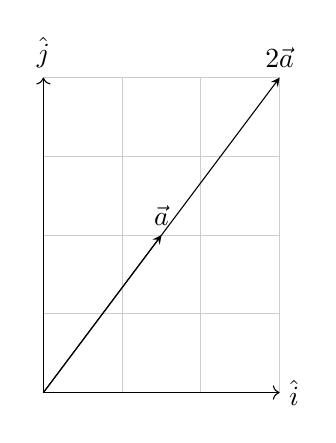
\begin{tikzpicture}
	\draw[thin,gray!40] (0,0) grid (3,4);
	\draw[.-> ] (0,0)--(3,0) node[right]{$\hat{i}$};
	\draw[.->] (0,0)--(0,4) node[above]{$\hat{j}$};
	\draw[.->,-stealth] (0,0)--(1.5,2)  coordinate (a)  node[above]{$\vec{a}$};
	\draw[.->,-stealth] (0,0)--(3,4) node[above]{$2\vec{a}$};
\end{tikzpicture}

\begin{itemize}
	\item 2 \emph{scales} the vector $\vec{a}$.
	So, 2 is a Scalar.
	\item Similarly basis vectors $\hat{i}$ and $\hat{j}$ can be scaled to represent any vector in 2d plane.
	
\end{itemize}

\hformbar
\formdesc{Span:}

\begin{itemize}

\item $a\vec{v}+b\vec{w}$ $\implies$ Linear combination of $\vec{v}$, $\vec{w}$

\item Set of all vectors of linear combination of $\vec{v}$, $\vec{w}$ ; $a\vec{v}+b\vec{w}$ is called \textbf{span}.


\item For most vectors span consists of all points on the plane.

\item If $\vec{v}$, $\vec{w}$ lie on same line, span is a line passin through origin.

\item If both $\vec{v}$, $\vec{w}$ are zero, span is zero.
\end{itemize}

\hformbar
\formdesc{Linear (in)dependent:}
\begin{itemize}
	\item If one vector can be represented as a linear combination of other, then the vectors are linearly dependent.
	\item A linearly dependent vector doesn't add to span of a vector.
	\item If one vector adds a dimension to a span of a vector, they are linearly independent.
\end{itemize}

\hformbar
\formdesc{Transformation:}
\begin{itemize}
	\item Takes a vector and gives a output vector.
\end{itemize}

\hformbar
\formdesc{Linear Transformation:}

The conditions for the tranformation to be linear are:

\begin{itemize}
	\item All lines must remain lines.
	\item Origin must be remain inplace.
	\item This makes all equidistant parallel lines remain equidistant and parallel.
	\item Matrices = Transformation of space.
	\item For example, the linear transform $\tctmat{1}{3}{-2}{0}$ transforms the 2d plane such a way that the new $\hat{i}$ lands at $\tcomat{1$\hat{i}$}{-2$\hat{j}$}$ and $\hat{j}$ lands at $\tcomat{3$\hat{i}$}{0$\hat{j}$}$
\end{itemize}

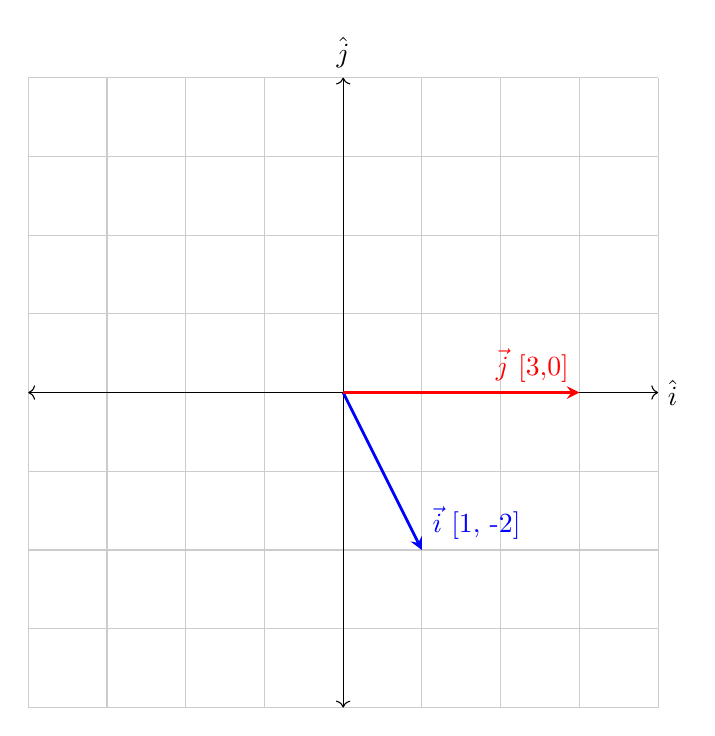
\begin{tikzpicture}
	\draw[thin,gray!40] (-4,-4) grid (4,4);
	\draw[<->] (-4,0)--(4,0) node[right]{$\hat{i}$};
	\draw[<->] (0,-4)--(0,4) node[above]{$\hat{j}$};
	\draw[line width=1pt,blue,-stealth](0,0)--(1,-2) node[anchor=south west]{$\vec{i}$	[1, -2]};
	\draw[line width=1pt,red,-stealth](0,0)--(3,0) node[anchor=south east]{$\vec{j}$	[3,0]};
\end{tikzpicture}
The new basis vectors are blue $\vec{i}$ and red $\vec{j}$.
\\
\\
Now in this new transformed space, every vector has to be represented as a linear combination of these two new basis vectors.
\\
\\
The vector $\vec{v} =$ -1$\hat{i} + 2 \hat{j}$ after transformation lands at the point $\tcomat{5}{2}$ in the new vector space.
\\
\\
Even after the transformation, the linear combination doesn't change. So, $\hat{i}$ and $\hat{j}$ are replaced by $\tcomat{1$\hat{i}$}{-2$\hat{j}$}$ and 	$\tcomat{3$\hat{i}$}{0$\hat{j}$}$ respectively.
\\
\\
So the new transformed $\vec{v}$ becomes,
\begin{equation}
	\vec{v}_{new}  = -1\hat{i}_{new} + 2 \hat{j}_{new}
\end{equation}
\begin{equation}
		\vec{v}_{new}  = -1\tcomat{1$\hat{i}$}{-2$\hat{j}$} + 2\tcomat{3$\hat{i}$}{0$\hat{j}$}
\end{equation}
\begin{equation}
			\vec{v}_{new}  =\tcomat{-1$\hat{i}$}{2$\hat{j}$} + \tcomat{6$\hat{i}$}{0$\hat{j}$}
\end{equation}

\begin{equation}
	\vec{v}_{new}  = \tcomat{5$\hat{i}$}{2$\hat{j}$}
\end{equation}
For any vector $x\hat{i}+y\hat{j}$, after applying the transformation $\begin{bmatrix}
	1 & 3\\
	$-2$ & 0
\end{bmatrix}$ becomes,
\begin{equation}
	 \begin{bmatrix}
		x \hat{i}\\
		y \hat{j}
		\end{bmatrix}  \overset{lr. \; transform}{ \implies }  x \begin{bmatrix}
		1 \hat{i}\\
		$-2$ \hat{j}
	\end{bmatrix} + y \begin{bmatrix}
	3 \hat{i}\\
	0 \hat{j}
\end{bmatrix} = \begin{bmatrix}
1x+3y \hat{i}\\
-2x+0y \hat{j}
\end{bmatrix} 
\end{equation}
Removing $\hat{i}$, $\hat{j}$ for legibility,
\begin{equation}
	\begin{bmatrix}
		x \\
		y 
	\end{bmatrix}  \overset{lr. \; transform}{ \implies }  x \begin{bmatrix}
		1 \\
		$-2$ 
	\end{bmatrix} + y \begin{bmatrix}
		3 \\
		0
	\end{bmatrix} = \begin{bmatrix}
		1x+3y\\
		-2x+0y
	\end{bmatrix} 
\end{equation}

This is the basis for Matrix multiplication.
\begin{itemize}
	\item $\begin{bmatrix}
		1 \\
		$-2$ 
	\end{bmatrix}$ is where $\hat{i}$ lands and $\begin{bmatrix}
	3 \\
	0 
\end{bmatrix}$ is where $\hat{j}$ (basis vectors) lands after the transformation.
\item So the 2X2 matrix $\begin{bmatrix}
	1 & 3\\
	$-2$ & 0
\end{bmatrix}$ itself can represent the transformation.
\item This explains the \emph{rules} for multiplication and why matrix multiplication is not commutative.
\item This also explains why the matrix $\begin{bmatrix}
	1 & 0\\
	0 & 1
\end{bmatrix}$ is an identity matrix. Since, this \emph{transform} actually does nothing, $\hat{i}$ and $\hat{j}$ remain unchanged.
\end{itemize}

For any transformation $\begin{bmatrix}
	a & b\\
	c & d
\end{bmatrix}$,
\begin{equation} \label{eq:transform1}\underbracket{
	 \begin{bmatrix}
		a & b\\
		c & d
	\end{bmatrix}}_{\mathclap{Transformation}} \overbracket{\begin{bmatrix}
	x\\
	y
\end{bmatrix}}^{old \; vector}=x  \overbracket{\begin{bmatrix}
a\\
c 
\end{bmatrix}}^{\mathclap{where \; \hat{i} \;  lands}} + y \underbracket{\begin{bmatrix}
b\\
d
\end{bmatrix}}_{\mathclap{where \; \hat{j} \; lands}} = \overbracket{\begin{bmatrix}
ax+by\\
cx+by
\end{bmatrix}}^{\mathclap{Transformed \; matrix}}
\end{equation}
\begin{itemize}
	\item $\begin{bmatrix}
		a\\
		c
	\end{bmatrix}$ and $\begin{bmatrix}
	b\\
	d
\end{bmatrix}$ are the new basis vectors; where old $\hat{i}$ and $\hat{j}$ land. These are the new transformed basis vectors.

\item Now these new basis vectors have to be used to represent all the vectors in it's span. In other words the linear combination of these two basis vectors.

\item From equation \ref{eq:transform1} it can be observed that the scalars $x$  and $y$ scale the corresponding new basis vectors.

	\item For no transformation (or) Identity transform / Multiplication,
	\begin{equation}
		\tctmat{1}{0}{0}{1} \tcomat{x}{y} = \tcomat{x}{y}
	\end{equation}
	Which makes sense !!
\end{itemize}

\hformbar
\formdesc{Counterclock Transform:}\\

$\tctmat{0}{-1}{1}{0}$ $\tcomat{x}{y}$


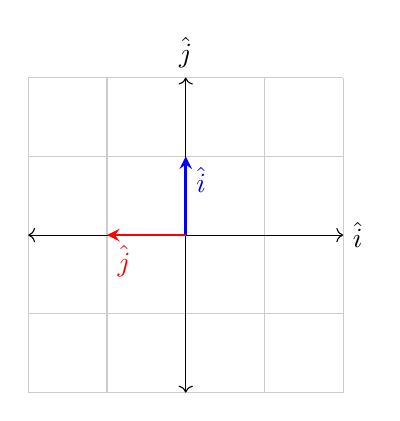
\begin{tikzpicture}
	\draw[thin,gray!40] (-2,-2) grid (2,2);
	\draw[<->] (-2,0)--(2,0) node[right]{$\hat{i}$};
	\draw[<->] (0,-2)--(0,2) node[above]{$\hat{j}$};
	\draw[line width=1pt,blue,-stealth](0,0)--(0,1.0) node[anchor=north west]{$\hat{i}$};
	\draw[line width=1pt,red,-stealth](0,0)--(-1,0) node[anchor=north west]{$\hat{j}$};
\end{tikzpicture}

\hformbar
\formdesc{Shear Transform:}\\

$\tctmat{1}{1}{0}{1}$ $\tcomat{x}{y}$


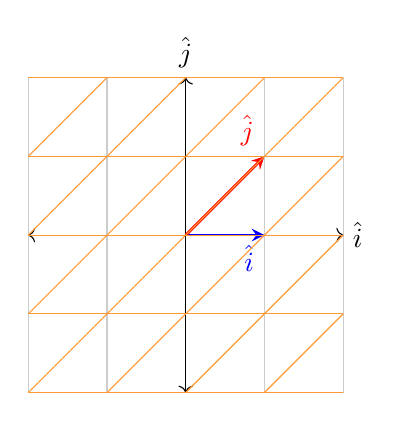
\begin{tikzpicture}
	\draw[thin,gray!40] (-2,-2) grid (2,2);
	\draw[<->] (-2,0)--(2,0) node[right]{$\hat{i}$};
	\draw[<->] (0,-2)--(0,2) node[above]{$\hat{j}$};
	\draw[line width=1pt,blue,-stealth](0,0)--(1,0) node[anchor=north east]{$\hat{i}$};
	\draw[line width=1pt,red,-stealth](0,0)--(1,1) node[anchor=south east]{$\hat{j}$};
	
%new grid
	%horizontal
	\foreach \y in {-2,...,2}
	{\draw[orange!80] (-2,\y)--(2,\y);}
	%vertical
	\draw[orange!80] (-2,1)--(-1,2);
	\draw[orange!80] (-2,0)--(0,2);
	\draw[orange!80] (-2,-1)--(1,2);
	\draw[orange!80] (-2,-2)--(2,2);
	\draw[orange!80] (-1,-2)--(2,1);
	\draw[orange!80] (0,-2)--(2,0);
	\draw[orange!80] (1,-2)--(2,-1);
\end{tikzpicture}

\hformbar
\formdesc{Few notable points:}\\

\begin{itemize}
	\newcommand\ii{$\tcomat{2}{1}$}
	\newcommand\jj{$\tcomat{-2}{-1}$}
	\item In transformations, order matters. $M_1M_2 \neq M_2M_1$ because $f(g(x)) \neq g(f(x))$
	\item The associative property $(AB)C = A(BC)$ holds true because the order is $C$, $B$ then $A$ regardless.
	\item For a $\tctmat{2}{-2}{1}{-1}$ transformation all 2d space is squished into a line.
	
	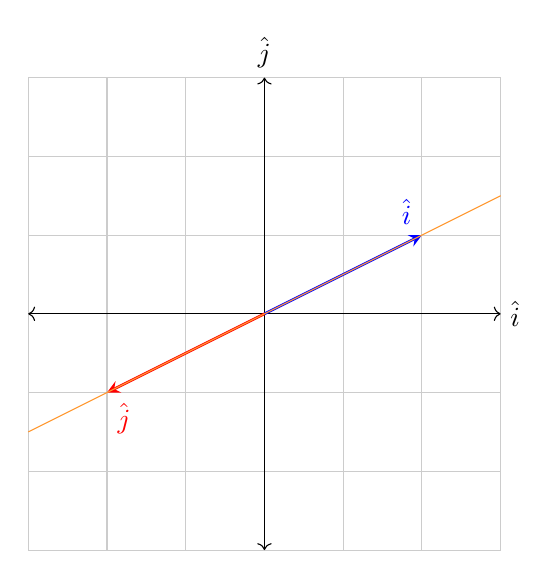
\begin{tikzpicture}
	\draw[thin,gray!40] (-3,-3) grid (3,3);
	\draw[<->] (-3,0)--(3,0) node[right]{$\hat{i}$};
	\draw[<->] (0,-3)--(0,3) node[above]{$\hat{j}$};
	\draw[line width=1pt,blue,-stealth](0,0)--(2,1) node[anchor=south east]{$\hat{i}$	\ii};
	\draw[line width=1pt,red,-stealth](0,0)--(-2,-1) node[anchor=north west]{$\hat{j}$	\jj};
	\draw[orange!80] (-3,-1.5)--(3,1.5);
	\end{tikzpicture}

These two vectors \ii and \jj are linearly dependent vectors.
\item Two transform for ex. shear and rotation can be composed into a single transform. This composition transform is nothing but a multiplication of shear and rotation matrix.
	\begin{equation}
	\underbracket{\tctmat{1}{1}{0}{1}}_{\mathclap{Shear}}
	\overbracket{ \tctmat{0}{-1}{1}{0}}^{\mathclap{Rotation}} \tcomat{x}{y} = 
	\underbracket{\tctmat{1}{-1}{1}{0}}_{\mathclap{Compostion}} \tcomat{x}{y}
	\end{equation}
\item Product or composition of two matrices/ transforms,
\begin{equation}
	\tctmat{a}{b}{c}{d} \tctmat{e}{f}{g}{h} = \tctmat{ae+bg}{af+bh}{ce+dg}{cf+dh}
\end{equation}

\end{itemize}

\hformbar
\formdesc{Determinant:}
\begin{itemize}
	\item Transformation $\tctmat{3}{0}{0}{2}$ scales $\hat{i}$ by factor 3 $\hat{j}$ by a factor 2.
		
	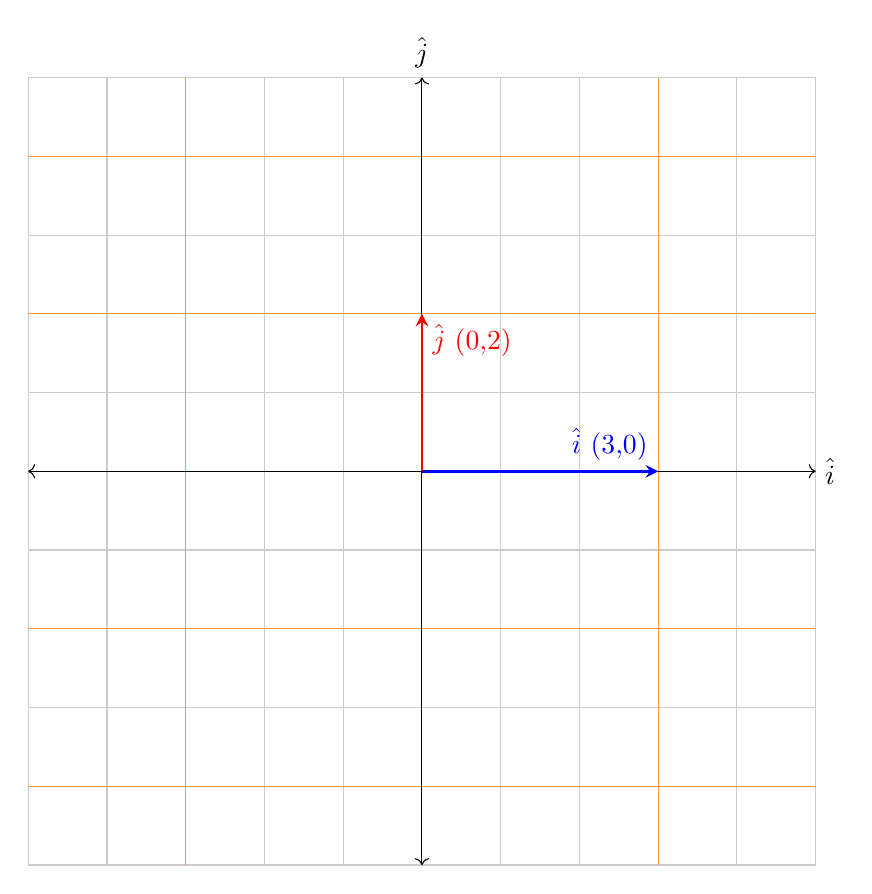
\begin{tikzpicture}
		\draw[thin,gray!40] (-5,-5) grid (5,5);
		% new grid
		\foreach \x in {-3,0,3}
		{\draw[orange!80] (\x,-5)--(\x,5);}
		\foreach \y in {-4,-2,...,4}
		{\draw[orange!80] (-5,\y)--(5,\y);}
		% axis
		\draw[<->] (-5,0)--(5,0) node[right]{$\hat{i}$};
		\draw[<->] (0,-5)--(0,5) node[above]{$\hat{j}$};
		% vector
		\draw[line width=1pt,blue,-stealth](0,0)--(3,0) node[anchor=south east]{$\hat{i}$ (3,0)};
		\draw[line width=1pt,red,-stealth](0,0)--(0,2) node[anchor=north west]{$\hat{j}$ (0,2)};
	\end{tikzpicture}

	\item We observe that the unit square in transformed space is scaled from 1 sq. unit to 3 sq. units. So the determinant of the transform/matrix $\tctmat{3}{0}{0}{2}$ is 3. In case of 3d, volume is scaled.
	\item For a matrix/transform $\tctmat{a}{b}{c}{d}$, the determinat is $ad-bc$.
	\item The determinant can be $-ve$ if the axis cross each other during the transformation. It has the effect of \emph{flipping} or \emph{inverting} the space.
	
	
	% Credit https://i.stack.imgur.com/0hxY1.png https://stackoverflow.com/a/34068511/4915164
	\begin{figure}[ht!]
		\graphicspath{ {images/math/} }
		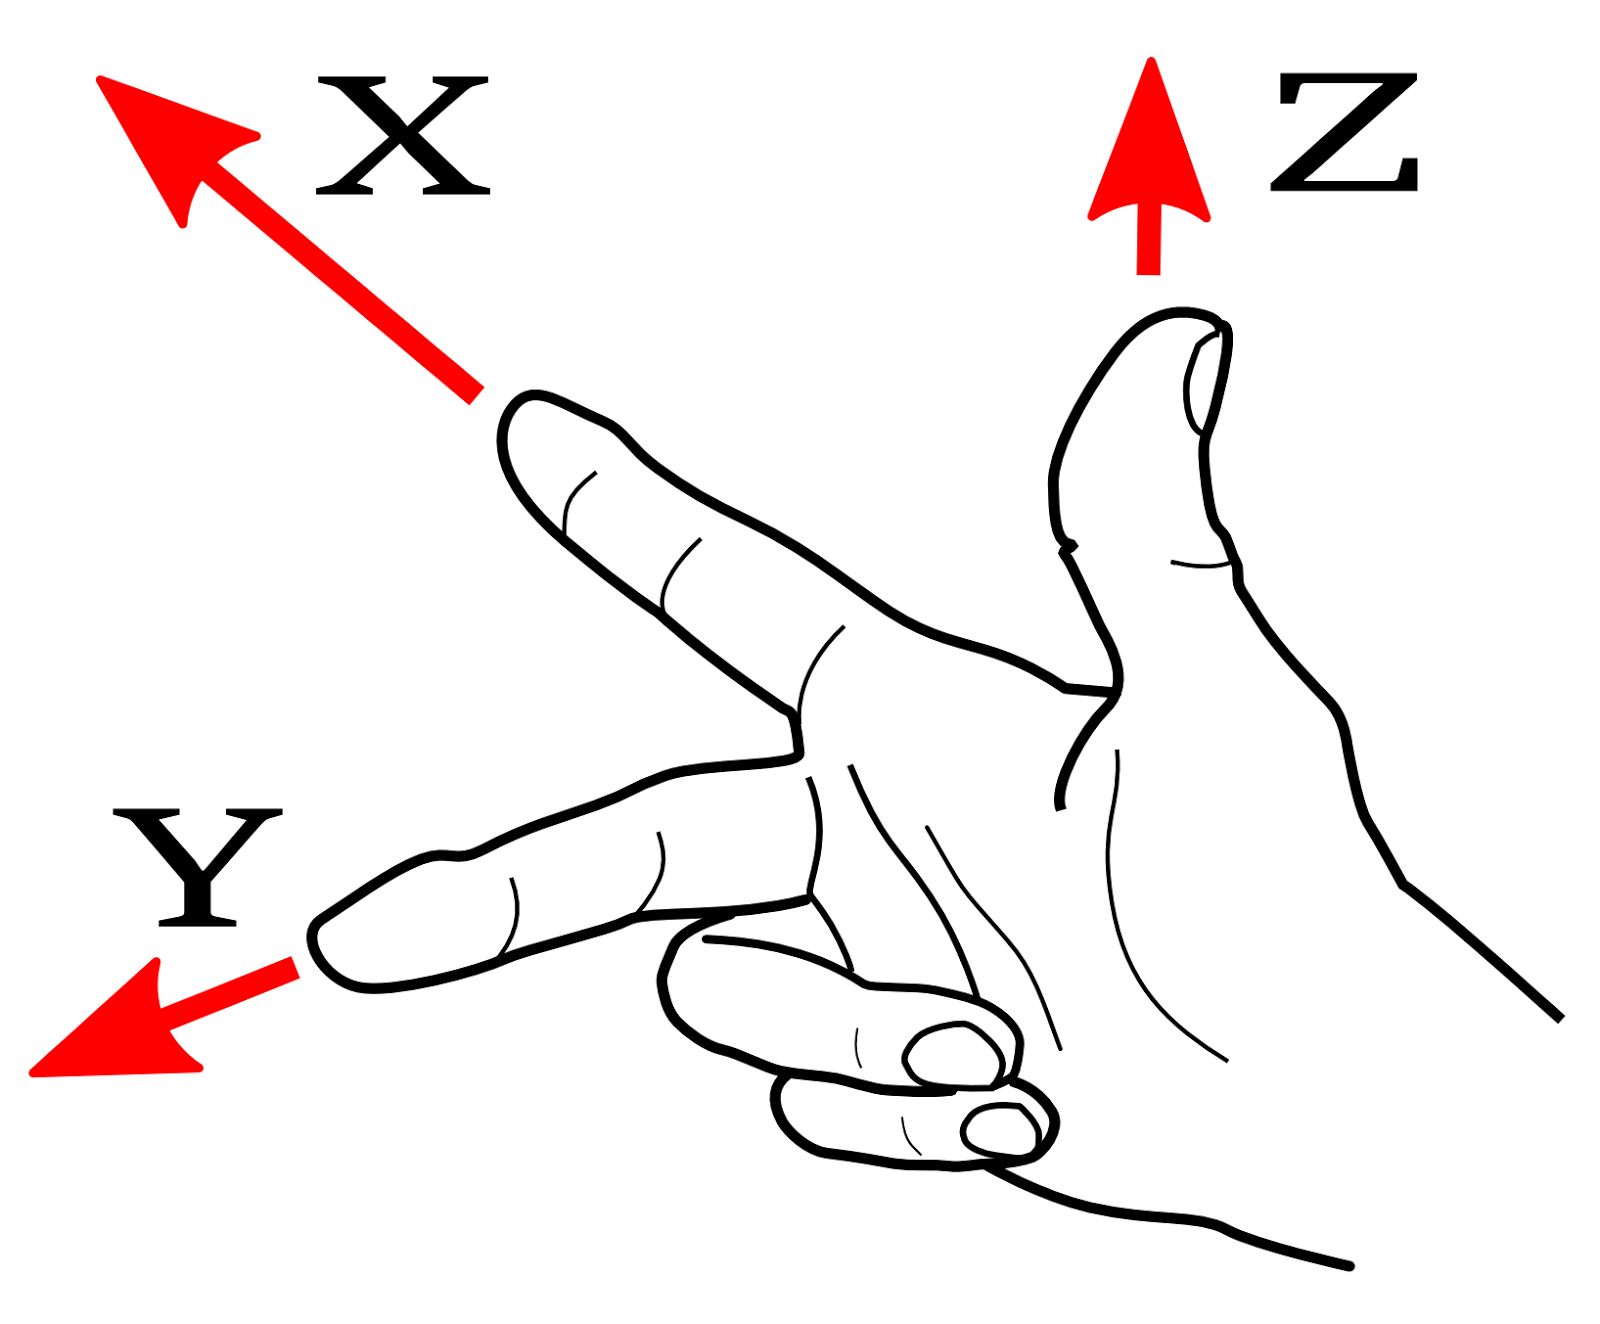
\includegraphics[width=\linewidth]{right-hand-rule.png}
	\end{figure}
	\item This can be checked using right hand rule to check if the axis still lie in the same orientation after transformation. If not, the determinant is $-ve$.
	\item For 3d space, determinant is measured by unit volume instead of area.
	\item Determinant can be zero if the space is squished. For ex. if transformed to a line or point in 2d or to a plane, line or a point in 3d. This has the effect of reduction in number of dimensions.
\end{itemize}

\begin{equation}
	det(M_1M_2) = det(M_1)  det(M_2)
\end{equation}


\hformbar
\formdesc{System of equations:}
\\


$A.\vec{X} = \vec{V}$\\

$3x+1y+4z = 1$

$3x+9y+2z = 6$

$3x+3y+3z = 8$

\begin{itemize}
	\item Solving these system of equations imply, finding the vector $\thcomat{x}{y}{z}$ that if applied the transformation $\thcthmat{3}{1}{4}{3}{9}{2}{3}{3}{3}$, would land on the vector $\thcomat{1}{6}{8}$.
	
	\item This can only be solved if $A^{-1}$ exists. Since space cannot be unpacked since there is/are lost dimension(s) if $det(A) = 0$. So $det(A) \neq 0$ has to be true for the system of equations to be solved using,
	
	\begin{equation}
		\vec{X} = A^{-1}\vec{V}
	\end{equation}
\end{itemize}

\hformbar
\formdesc{Rank:}
\begin{itemize}
	\item Rank is the number of dimensions of the transformed space.
	\item The Rank of a matrix ; output space.
	
	Rank : 1 $\implies$ output transformation : Line
	
	Rank : 2 $\implies$ output transformation : Plane
	
	Rank : 0 $\implies$ output transformation : Point
\end{itemize}


\hformbar
\formdesc{Column space:}

\begin{itemize}
	\item Set of all possible linear combinations or span of column vectors of $A$. Or,
	\item Set of all possible $A \vec{V}$
\end{itemize}

\hformbar
\formdesc{Null space:}
\begin{itemize}
	\item Set of vectors that get squished into origin after transformation.
\end{itemize}

\hformbar
\formdesc{Dot Product:}
\begin{itemize}
	\item $\vec{a}$ and $\vec{b}$ are two vectors and angle between them is $\theta$.
	
	\begin{equation}
		\vec{a} = [a_1 ,a_2 ,... a_n]
	\end{equation}
	\begin{equation}
		\vec{b} = [b_1, b_2,... b_n]
	\end{equation}
	\begin{equation}
		\vec{a}.\vec{b} = (a_1)*(b_1) + (a_2)*(b_2) + ... + (a_n)*(b_n)
	\end{equation}
	
	\item Geometric representation:
	\begin{equation}
		\vec{a}.\vec{b} = ||{a}||* ||{b}||* cos \theta
	\end{equation}
	
	\begin{tikzpicture}
		\coordinate (o) at (0,0);
		\draw[.->] (0,0)--(5,0)  coordinate (a) node[right]{$\vec{a}$};
		\draw[.->] (0,0)--(3,4)  coordinate (b)  node[above]{$\vec{b}$};
		\pic [draw, ->, "$\theta$", angle eccentricity=1.5] {angle =a--o--b};
	\end{tikzpicture}
	
	dot product of two vectors = (length of any vector) x 
	(length of projection made on the vector)
	
\end{itemize}


\newcommand{\dotbase}{
	\coordinate (o) at (0,0);
	\draw[thin,gray!40] (-2,-2) grid (6,4);
	\draw[<->] (-2,0)--(6,0) node[right]{$\hat{i}$};
	\draw[<->] (0,-2)--(0,4) node[above]{$\hat{j}$};
	\draw[line width=1pt,blue,-stealth](0,0)--(2,2) coordinate (a) node[anchor=south east, pos=0.8]{$\vec{a}$	[2,2]};
	\draw[line width=1pt,red,-stealth](0,0)--(4,-1) coordinate (b) node[anchor=south west]{$\vec{b}$	[4,-1]};
	\pic [draw, ->, "$\theta$", angle eccentricity=1.5] {angle =b--o--a};
}

\begin{tikzpicture}
	\dotbase
\end{tikzpicture}
\\
\\

Projecting $\vec{a}$ on $\vec{b}$:

\begin{tikzpicture}
	\dotbase
	\draw[dashed] (2,2)--(1.411764,-0.352941176) coordinate(p);
	\draw [decorate,decoration={brace,amplitude=10pt,mirror,raise=2pt},yshift=0pt]
	(0,0) -- (1.411764,-0.352941176) node [black,midway,xshift=0pt, yshift=-25pt,rotate=-13] {\footnotesize
		length of projection};
        \tkzMarkRightAngle[draw=black,size=.2](o,p,a);
        
\end{tikzpicture}

\begin{itemize}
	\item Length of projection = $a.cos\theta$
	\item Dot product = $a .cos\theta . b$
	\item The length of projection does not depend on the length of $\vec{b}$. It only depends on length of $\vec{a}$ and $\theta$.
	\item Projecting $\vec{b}$ on $\vec{a}$ will result in the same dot product result. The order does not matter.
	\item If projection does not lie betweeon origin and the end point of the other vector, you can extend the other vector since length of projection is not affected by it.
	\item Dot product is -ve if projection is on -ve side.
\end{itemize}

\hformbar
\formdesc{Cross Product:}

\begin{itemize}
	\item Directed area product.
	%https://en.wikipedia.org/wiki/Cross_product#/media/File:Cross_product_parallelogram.svg
		\begin{figure}[ht!]
		\graphicspath{ {images/math/} }
		\includesvg[width=\linewidth]{cross_product_parallelogram}
	\end{figure}

	% https://en.wikipedia.org/wiki/Cross_product#/media/File:Right_hand_rule_cross_product.svg
	\begin{figure}[ht!]
		\graphicspath{ {images/math/} }
		\includesvg[width=\linewidth]{right_hand_rule_cross_product}
	\end{figure}

	\item $\vec{a}\times \vec{b} = -\vec{b} \times \vec{a}$
	\item Length of $\vec{a}\times \vec{b}$ = $det (\tctmat{$a_1$}{$b_1$}{$a_2$}{$b_2$})$
	\item The cross product vector is normal to the area.
	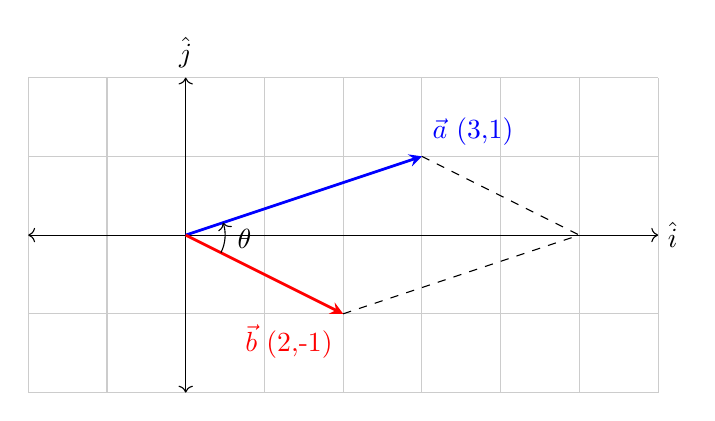
\begin{tikzpicture}
		\coordinate (o) at (0,0);
		\draw[thin,gray!40] (-2,-2) grid (6,2);
		\draw[<->] (-2,0)--(6,0) node[right]{$\hat{i}$};
		\draw[<->] (0,-2)--(0,2) node[above]{$\hat{j}$};
		\draw[line width=1pt,blue,-stealth](0,0)--(3,1) coordinate (a) node[anchor=south west]{$\vec{a}$	(3,1)};
		\draw[line width=1pt,red,-stealth](0,0)--(2,-1) coordinate(b) node[anchor=north east]{$\vec{b}$	(2,-1)};
		\draw[dashed] (2,-1)--(5,0);
		\draw[dashed] (3,1)--(5,0);
		\pic [draw, ->, "$\theta$", angle eccentricity=1.5] {angle =b--o--a};
	\end{tikzpicture}
	\item The area of this parallelogram is $det (\tctmat{3}{2}{1}{-1})$
	\item The direction of the cross product is normal to the area, i.e, in the direction of $\hat{k}$
	\item The magnitude of this vector is the area of this parallelogram i.e, determinant.
	\begin{equation}
		\vec{a} \times \vec{b} = ||a|| . ||b|| sin\theta
	\end{equation}
\end{itemize}


\hformbar
\formdesc{Eigen:}
\begin{itemize}
	\item For a few transformations, vectors only scale. i.e, only stretch or compress.
	\item Such vectors are called eigen vectors of the transformation.
	\item Such vectors are transformed into it's own span.
	\item The scaled value of such vectors (scalar) is the eigen value. It can be +ve or -ve.
	\begin{equation}
		A\vec{V} = \lambda \vec{V}
	\end{equation}
where:

	$A$ is the transformation,
	
	$\vec{V}$ is the eigen vector and,
	
	$\lambda$ is the eigen value.
\end{itemize}


\hformbar
\formdesc{Vector from origin:}\\
\begin{itemize}
	\item As discussed previously, any vector can be moved to origin for reference, without changing it's direction it is pointing to and it's length.
	\item To make a vector starting from $\thcomat{$a_1$}{$a_2$}{$a_3$}$ and ending at $\thcomat{$b_1$}{$b_2$}{$b_3$}$ as a reference vector, we can apply triangular law of addition to get a vector which starts from origin and is equivalent with the vector starting and ending at the above two points.
	\item We need to remember that the above vectors themselves start at origin. So, we can get the vector by doing $\thcomat{$a_1$}{$a_2$}{$a_3$}$ $-$ $\thcomat{$b_1$}{$b_2$}{$b_3$}$
\end{itemize}

\hformbar
\formdesc{Matrices:}\\

Diagonal Matrix:
\begin{itemize}
	\item A matrix with all 0's except diagonal elements.
\end{itemize}

\hformbar

Identity Matrix:
\begin{itemize}
	\item A Matrix with all diagonal elements as 1.
	
	$I = \thcthmat{1}{0}{0}{0}{1}{0}{0}{0}{1}$
\end{itemize}

\hformbar

Scalar Matrix:
\begin{itemize}
	\item A Matrix with only equal diagonal elements.
	\item A scalar matrix can be represented by a single scalar.
	
	$K.I = \thcthmat{4}{0}{0}{0}{4}{0}{0}{0}{4}$
\end{itemize}
\hformbar

Upper Triangular Matrix:
\begin{itemize}
\item A Matrix with all elements below diagonal are 0

$\thcthmat{3}{5}{2}{0}{2}{7}{0}{0}{1}$
\end{itemize}

\hformbar

Lower Triangular Matrix:
\begin{itemize}
	\item A Matrix with all elements above diagonal are 0
	
	$\thcthmat{3}{0}{0}{7}{2}{0}{5}{3}{1}$
\end{itemize}

\hformbar

Symmetric Matrix:
\begin{itemize}
	\item A square matrix which is equal to its transpose.
	\item $A=A^T$
	\item $a_{ij} = a_{ji}$ for every i and j.
	
%https://en.wikipedia.org/wiki/Symmetric_matrix#/media/File:Matrix_symmetry_qtl1.svg
	\begin{center}
		\graphicspath{ {images/math} }
		\includesvg[width=\linewidth]{matrix_symmetry.svg}
	\end{center}

\end{itemize}


\hformbar

Skew Symmetric Matrix:
\begin{itemize}
	\item A square matrix which is equal to negative of its transpose.
	\item $A=-A^T$
	\item $a_{ij} = -a_{ji}$ for every i and j.
\end{itemize}


\hformbar

Orthogonal Matrix:
\begin{itemize}
	\item A square matrix whose column vectors and row vectors are orthonormal.
	\item $AA^T=A^TA=I$ or,
	\item $A^T=A^{-1}$
	\item $a_{ij} = -a_{ji}$ for every i and j.
\end{itemize}


\hformbar
\formdesc{Lines, Planes and Hyperplanes:}\\


\end{document}